
\documentclass[11pt]{article}
\usepackage{../../Shared_Resources/Latex_Styles/General_Style} 
\usepackage{../../Shared_Resources/Latex_Styles/mcode} 

\usepackage{listings}

\lstset{ frame=single}

\begin{document}

\lstset{frameround=fttt,language=Matlab}

\lstMakeShortInline[columns=fixed]|

\makeheader{1 -- September 22, 2021}{Solutions -- Introduction to \Matlab/Octave}


{\bf{Solution I (MATLAB)}}\\

We consider the following MATLAB code:

%%\lstinputlisting{../build/solution/solution1.m}

\bigskip

{\bf{Solution II (MATLAB)}}\\

\begin{enumerate}

\item We consider the following MATLAB script |logplot.m|:

%%\lstinputlisting{../build/solution/solution2.m}

\item For the function $f(x) = [x - \log(x+1)]^4$, we have that:

\[
\log(f(x)) = 4 \log(x-\log(x+1)) \quad 
\begin{cases} 
      \leq 4\log x \\
      \geq 4 \log(x-7) \, , 
\end{cases}
\text{for} \, x \in [0, 1000],
\]
so that the curve $(x,f(X))$ is close to a straight line in the plot with the logarithmic scale on both the axes; its slope is approximately $p=4$, being $f(x)=\mathcal{O}(x^p)$. Therefore, the plot obtained with the command |loglog| is the most useful to estimate the order of growth of $f(x)$.

\item We add the following MATLAB commands to the code suggested in a) to obtain the indicated figure:
%%\lstinputlisting{../build/solution/solution2_c.m}

\end{enumerate}


{\bf{Solution III (MATLAB)}}\\

\begin{enumerate}

\item Since we conjecture that the error reads $E_{c,h_i}=C h_i^p$, then we have that $\log E_{c,h_i} = \log C + p\log h_i$, for $h = 1, \ldots, n$. Therefore, when using a logarithmic scale on both axes (\textit{log-log scale}) for plotting the errors $E_{c,h_i}$ vs. $h_i$, we should obtain a straight line $\log E_{c,h_i}$ of slope $p$, where $p$ is the order of convergence. In order to graphically determine $p$, we plot the errors $E_{c,h_i}$ vs. $h_i$ in log-log scale and compare the line obtained with those corresponding to the lines $(h_i,h_i^q)$ for some values of $q$, e.g. $q=1,2,3$. The value of $q$ for which $(h_i,h_i^q)$ is \textit{parallel} in log-log scale to $(h_i,E_{c,h_i})$ corresponds to the convergence order of the method $p$. We use the following MATLAB commands to \textit{graphically} determine $p$:
%% \lstinputlisting{../build/solution/solution3.m}
%% \begin{figure}[!h]
%%   \centering
%% 	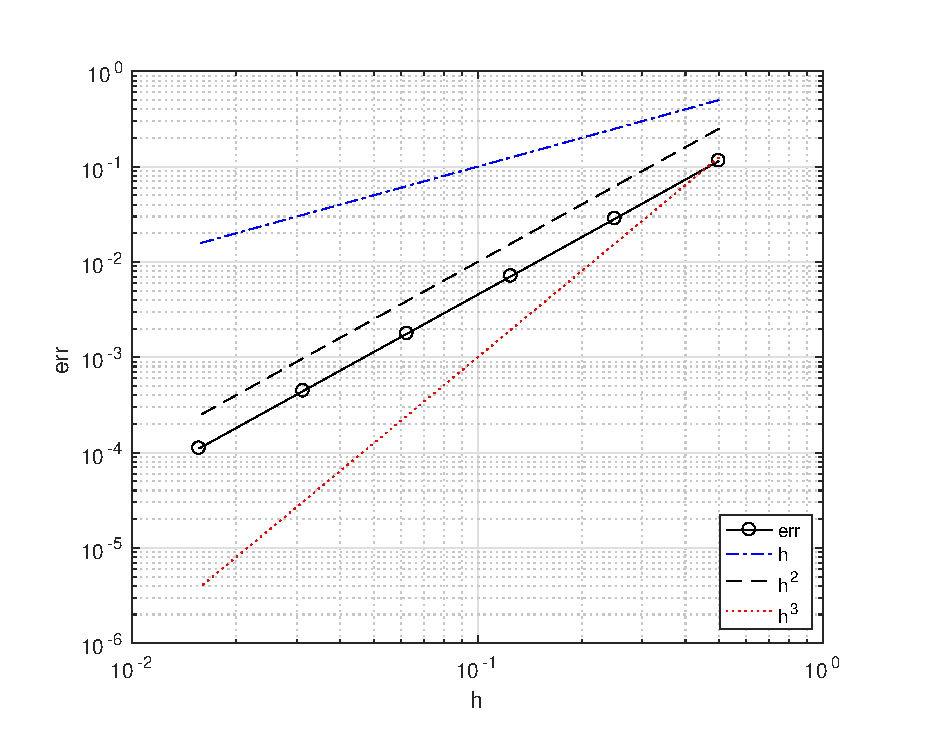
\includegraphics[width=\textwidth]{../figures/solution3.eps}
%% \end{figure}
\FloatBarrier
We deduce that the convergence order of the method is $p=2$ since $(h_i,E_{c,h_i})$ is \textit{parallel} to $(h_i,h_i^2)$ in the log-log scale plot.

We remark that in practical cases the conjecture $E_{c,h_i}=C h_i^p$ can be typically used only for ``small'' values of $h_i (h_i \rightarrow 0)$, for which it suffices to verify that the lines $(h_i,E_{c,h_i})$ and $(h_i,h_i^p)$ in log-log scale are parallel in the left part of the previous plot.
\FloatBarrier
\item Still using the conjecture $E_{c,h_i}=C h_i^p$, let us consider the errors $E_{c,h_{i-1}}=C h_{i-1}^p$ and $E_{c,h_i}=C h_i^p$ corresponding to $h=h_{i-1}$ and $h_i$ for $i=2, \ldots , n$, respectively. Then, we have:
\begin{align*}
\frac{E_{c,h_i}}{E_{c,h_{i-1}}} = \left( \frac{h_i}{h_{i-1}} \right)^p \, , \qquad p = \frac{\log \left( \frac{E_{c,h_i}}{E_{c,h_{i-1}}} \right)}{\log \left( \frac{h_i}{h_{i-1}} \right)} \qquad \text{for} \, \, i = 2, \ldots, n.
\end{align*}
Since in practical cases the conjecture $E_{c,h_i}=C h_i^p$ holds for  ``small'' values of $h_i$, we typically select $i=n$ to determine the convergence order of the method $p$:
\begin{align*}
p = \frac{\log \left( \frac{E_{c,h_n}}{E_{c,h_{n-1}}} \right)}{\log \left( \frac{h_n}{h_{n-1}} \right)}.
\end{align*}
We use the following MATLAB command to \textit{algebraically} determine that $p=2$:
%% \lstinputlisting{../build/solution/solution3_c.ms}
\end{enumerate}

\bigskip

{\bf{Solution IV (MATLAB)}}\\

We use the MATLAB commands:
%%\lstinputlisting{../build/solution/solution4.m}
\begin{enumerate}
\item We extract the element in position (1,3) (first row, third column) as:
%%\lstinputlisting{../build/solution/solution4_a.m}
\item We extract the second row as:
%%\lstinputlisting{../build/solution/solution4_b.m}
\item We extract the first two columns from the matrix as:
%%\lstinputlisting{../build/solution/solution4_c.m}
\item We extract the vector containing all the elements of the second row of the matrix except for the third element as:
%%\lstinputlisting{../build/solution/solution4_d.m}
\end{enumerate}

\bigskip

{\bf{Exercise V (MATLAB)}}\\
We use the following MATLAB code:
%%\lstinputlisting{../build/solution/solution5.m}

We can clearly see that the expression $f(x) = (\sqrt{1+x}-1)/x$ suffers from severe round-off errors as $x$ approaches machine precision, because we compute the difference of two numbers with similar values, $\sqrt{1+x}$ and $x$, which causes a cancellation of significant digits (\textit{hint}: type |eps| in the console to visualize the best relative precision that you can get using MATLAB).


































\end{document}
